\documentclass[tikz,border=10pt]{standalone}
\usetikzlibrary{intersections, calc}

\begin{document}
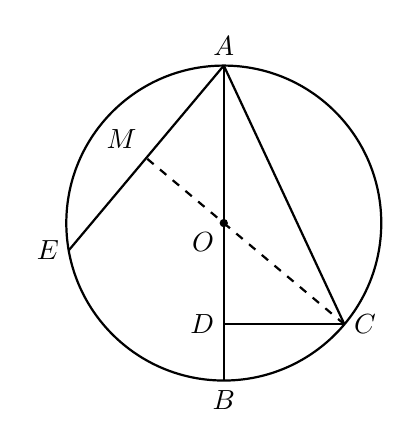
\begin{tikzpicture}
    % 1. 定义基本参数
    \def\r{2} % 半径
    \coordinate (O) at (0,0);
    
    % 2. 绘制圆
    \draw[thick] (O) circle (\r);
    \fill (O) circle (1.5pt) node[below left] {$O$};
    
    % 3. 定义关键点坐标
    \coordinate (A) at (90:\r);
    \coordinate (B) at (270:\r);
    \coordinate (C) at (320:\r);
    \coordinate (E) at (190:\r);
    
    % 4. 计算辅助点 D：C 在直径 AB 上的垂足
    \coordinate (D) at ($(A)!(C)!(B)$);
    
    % 5. 绘制直径 AB
    \draw[thick] (A) -- (B);
    
    % 6. 绘制其他线条
    \draw[thick] (A) -- (E);
    \draw[thick] (A) -- (C);
    \draw[thick] (D) -- (C);
    
    % 7. 延长 OC 与 AE 相交于 M（你要的修改）
    \path[name path=AE] (A) -- (E);
    \path[name path=OC_extend] (C) -- ($(O)!-1.5!(C)$); % 反向延长OC
    \path[name intersections={of=AE and OC_extend, by=M}]; % 求交点M
    \draw[dashed, thick] (C) -- (M); % 虚线OC延长到M
    
    % 8. 标注标签
    \node[above] at (A) {$A$};
    \node[below] at (B) {$B$};
    \node[right] at (C) {$C$};
    \node[left] at (E) {$E$};
    \node[left] at (D) {$D$};
    \node[above left] at (M) {$M$}; % 标注M
    
\end{tikzpicture}
\end{document}